% Chapter 2: Background and Related Work
Before explaining the details and implementation of the methodology used in the context of this thesis, it is essential to provide an overview of the evolution of the inner workings of the Transformer architecture as well as Language Models in general. In addition, in this chapter covers relevant optimization techniques and how they influenced the final result.
Finally, we will also shed some light on the target hardware, whose limitations have been a driving force behind the design choices made in this project.

\section{Early Language Models}
Before the emergence of the Transformer architecture, language models predominantly relied on \textit{Recurrent Neural Networks} (RNNs) . These networks represent an evolution of the \textit{Multi-Layer Perceptron} (MLP), incorporating cyclic connections within their architecture to create recurrent circuits. This design enables the network to maintain a form of memory, allowing it to consider previous inputs when generating predictions and thereby capturing long-range dependencies inherent in sequential data such as text.

Despite their theoretical advantages, RNNs suffer from a critical limitation known as the vanishing gradient problem \cite{rnn}. During backpropagation, throughout time, gradients from earlier steps diminish exponentially as they propagate backward through the network layers. This degradation severely hampers the network's ability to be trained effectively, as the influence of distant past information becomes negligible in the parameter updates.

To address these limitations, Hochreiter and Schmidhuber introduced \textit{Long Short-Term Memory} (LSTM) networks \cite{lstm}, which revolutionized sequence modeling through their sophisticated gating mechanisms. LSTMs employ specialized memory cells designed to selectively retain, update, and output information across extended sequences. The architecture incorporates three fundamental gate types that regulate information flow:
\begin{itemize}
    \item The \textit{input gate} determines the extent to which new information from the current input should be incorporated into the cell state. It evaluates the relevance of incoming data and controls its integration with existing memory.
    \item The \textit{forget gate} governs the retention of information from previous time steps, deciding which aspects of the historical cell state remain relevant and should be preserved.
    \item Finally, the \textit{output gate} regulates how much of the current cell state should be exposed to subsequent layers, effectively controlling what information propagates forward in the network.
\end{itemize}

This gating mechanism allows LSTMs to maintain gradient flow over much longer sequences compared to vanilla RNNs. Thus, they can capture dependencies spanning hundreds of time steps, making them particularly effective for tasks requiring long-term context understanding such as language modeling, machine translation, and text summarization. A visual representation of an LSTM cell is shown in Figure \ref{fig:lstm-architecture}.
\begin{figure}[!htbp]
\centering
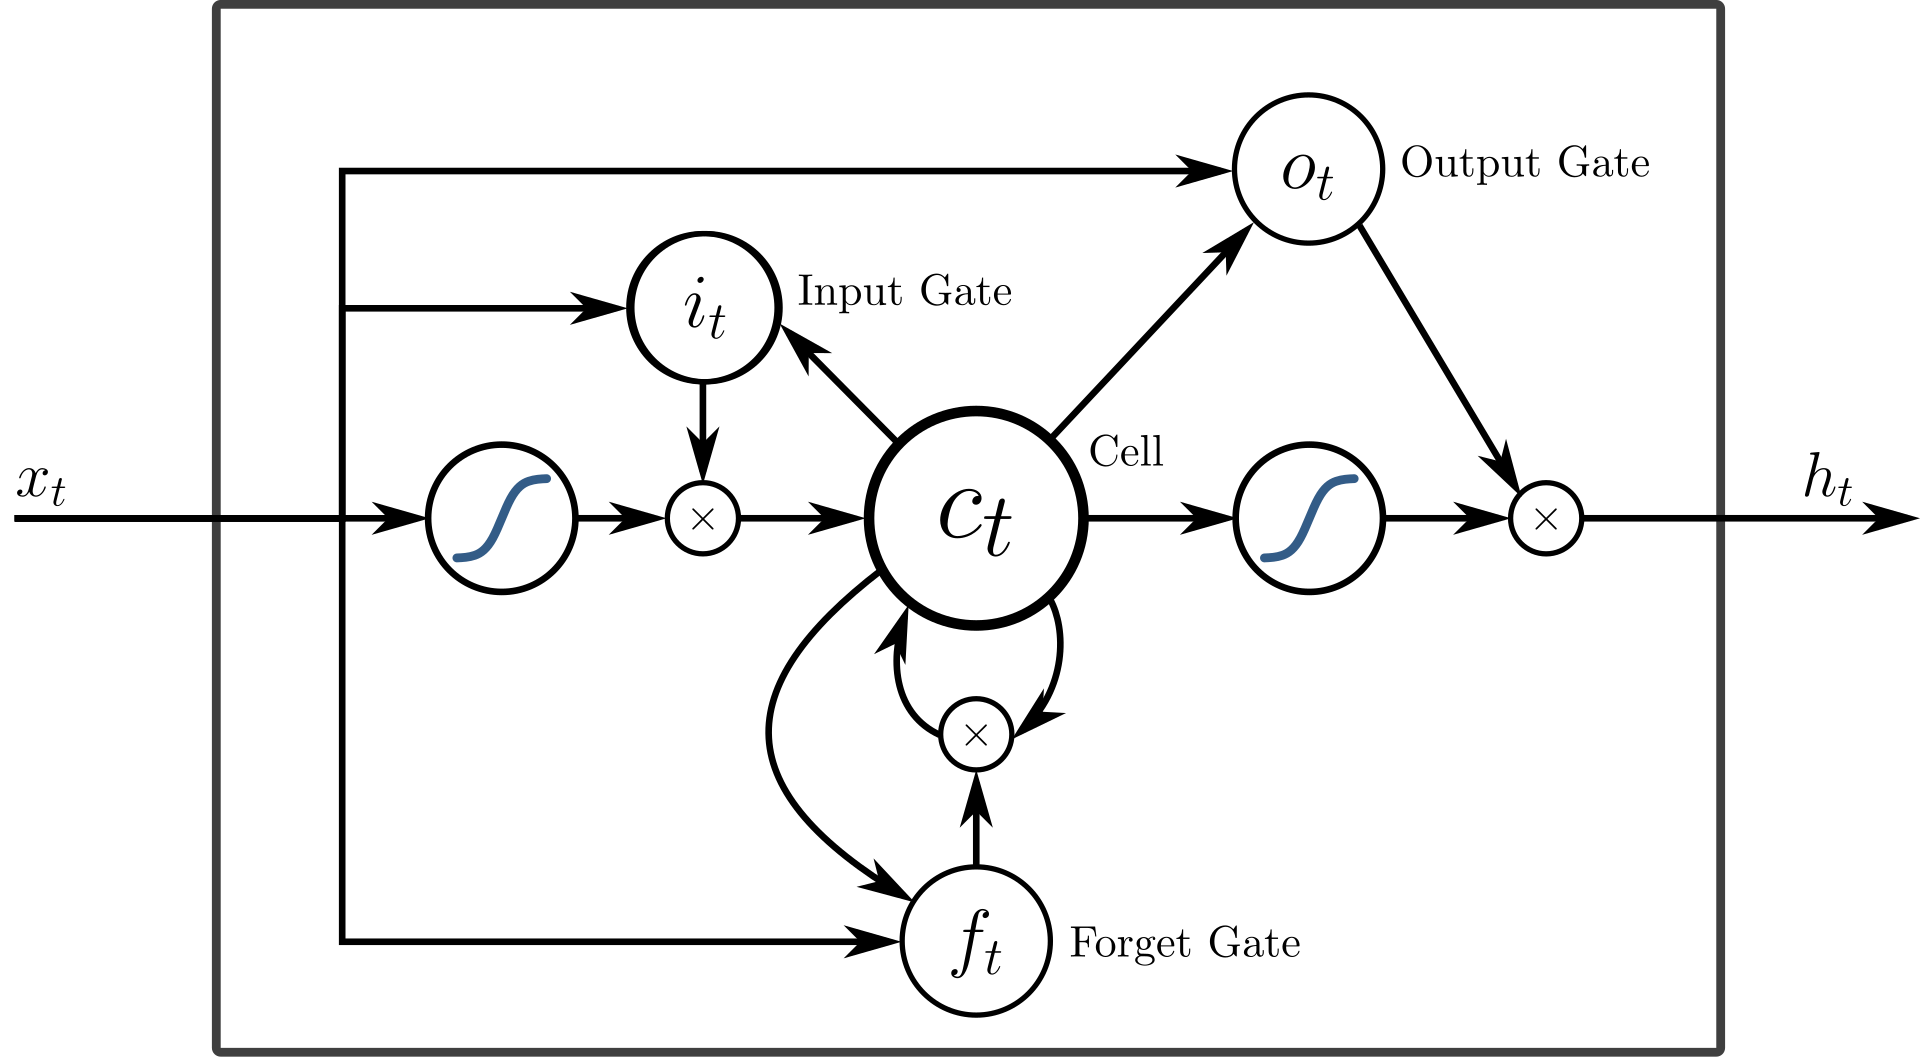
\includegraphics[width=0.7\textwidth]{image.png}
\caption{Architecture of an LSTM cell showing the three gating mechanisms. The input gate (left) controls information incorporation, the forget gate (center) manages memory retention, and the output gate (right) regulates information flow to subsequent layers. The cell state (horizontal line) maintains long-term memory throughout the sequence.}
\label{fig:lstm-architecture}
\end{figure}

While LSTMs significantly improved the ability to model sequential data, they still faced challenges in terms of parallelization and context understanding, especially when compared to Transformers.  Nevertheless, LSTMs are still widely used for various \textit{natural language processing} (NLP) tasks, including text generation \cite{lstm_textgeneration}.

\section{The Transformer Architecture}  \label{transformer_architecture}

The Transformer architecture, introduced by Vaswani et al. \cite{attention_is_all_you_need}, fundamentally changed how we approach sequence modeling by abandoning recurrent connections entirely in favor of attention mechanisms. Unlike LSTMs that process sequences step-by-step, the Transformer can examine all positions simultaneously, allowing for efficient parallelization during training. Moreover, it can capture long-range dependencies thanks to the attention mechanism.

\subsection{The Attention Mechanisms}

At the core of the Transformer lies the attention mechanism, which fundamentally changed how neural networks process sequential information. The attention mechanism addresses the information bottleneck created when sequence models compress an entire input sequence into a single fixed-size vector. This bottleneck becomes particularly problematic for long sequences, where important information can be lost or diluted.

Attention allows a model to dynamically focus on different parts of the input sequence when generating each output token, similar to how humans selectively concentrate on relevant information when reading or translating text. This is done, essentially, by directly comparing and relating any two positions in a sequence, regardless of their distance (i.e. self-attention). This selective focus mechanism enables the model to capture long-range dependencies more effectively and provides interpretable insights into which input elements influenced specific predictions.

\subsection{Scaled Dot-Product Attention Mechanics}

The Transformer's scaled dot-product attention operates on three matrices derived from the input:

\begin{equation}
\text{Attention}(Q, K, V) = \text{softmax}\left(\frac{QK^T}{\sqrt{d_k}}\right)V
\end{equation}

Each component serves a specific purpose:

\begin{itemize}
   \item \textbf{Queries (Q)}: Generated by $Q = XW_Q$ where $X$ is the input and $W_Q \in \mathbb{R}^{d_{\text{model}} \times d_k}$. Each query vector represents ``what information am I looking for?''
   \item \textbf{Keys (K)}: Generated by $K = XW_K$ where $W_K \in \mathbb{R}^{d_{\text{model}} \times d_k}$. Keys act as indexed labels for each position's content.
   \item \textbf{Values (V)}: Generated by $V = XW_V$ where $W_V \in \mathbb{R}^{d_{\text{model}} \times d_v}$. Values contain the actual information to be retrieved.
\end{itemize}

The attention computation proceeds in four steps:

\begin{enumerate}
   \item \textbf{Similarity Computation}: $QK^T$ produces a $n \times n$ matrix where entry $(i,j)$ represents how much position $i$ should attend to position $j$. The dot product naturally measures similarity between query and key vectors.

   \item \textbf{Scaling}: Division by $\sqrt{d_k}$ (where $d_k$ is the dimensionality of the keys) prevents the dot products from becoming too large. Without scaling, large dot products push the softmax function into regions with extremely small gradients. For example, if $d_k = 512$, dot products could reach magnitudes of $\pm 20$ or more, causing softmax to output distributions close to one-hot vectors.

   \item \textbf{Normalization}: The softmax function converts similarity scores into a probability distribution: $\text{softmax}(x_i) = \frac{e^{x_i}}{\sum_{j=1}^n e^{x_j}}$. This ensures attention weights sum to 1 and creates a differentiable selection mechanism.

   \item \textbf{Weighted Aggregation}: The attention weights are applied to the value vectors, producing a weighted sum that represents the attended information for each position.
\end{enumerate}

\subsection{Multi-Head Attention Architecture}

The Transformer employs multi-head attention so that each head can focus on different parts of the input. Some heads might track syntax, others semantics, positions, etc. This is done by projecting the input matrices $Q, K, V$ by $h$ times using different learned linear projections:
\begin{equation}
(QW_i^Q, KW_i^K, VW_i^V)
\end{equation}
Given this, each head is computed as:
\begin{equation}
\text{head}_i = \text{Attention}(QW_i^Q, KW_i^K, VW_i^V)
\end{equation}
As such, the final equation for multi-head attention is:
\begin{equation}
\text{MultiHead}(Q, K, V) = \text{Concat}(\text{head}_1, \ldots, \text{head}_h)W^O
\end{equation}

Each head uses different projection matrices $W_i^Q \in \mathbb{R}^{d_{\text{model}} \times d_k}$, $W_i^K \in \mathbb{R}^{d_{\text{model}} \times d_k}$, and $W_i^V \in \mathbb{R}^{d_{\text{model}} \times d_v}$, where typically $d_k = d_v = d_{\text{model}}/h$ for $h$ heads. 

Multi-head attention essentially gives the model multiple different perspective of the same input, and it is a vital system that contributes to make this architecture so powerful.

\subsection{Positional Information Integration}

Since attention is permutation-invariant, the Transformer requires explicit positional information. The original work uses sinusoidal positional encodings:

\begin{align}
PE_{(\text{pos}, 2i)} &= \sin(\text{pos}/10000^{2i/d_{\text{model}}}) \\
PE_{(\text{pos}, 2i+1)} &= \cos(\text{pos}/10000^{2i/d_{\text{model}}})
\end{align}

These encodings have useful properties: they create unique representations for each position, allow the model to learn relative positions through linear combinations, and can theoretically handle sequences longer than those seen during training.

This architecture enables the Transformer to model dependencies between any pair of positions with constant path length, while maintaining full parallelizability during training.

\subsection{Encoder-Decoder Transformers}

Transformer-based models generate text by predicting the next token in a sequence, conditioned either on an external input (encoder-decoder models) or on the sequence generated so far (decoder-only models). The former is what the original Transformer architecture~\cite{attention_is_all_you_need} follows.

\begin{itemize}
  \item The \textbf{encoder} processes the full input sequence in parallel, producing a series of contextual embeddings that capture the meaning and structure of the input tokens.
  \item The \textbf{decoder} generates the output sequence token by token, using the embeddings from the encoder.
\end{itemize}

This design enables the model to generate outputs that are grounded in the input sequence, rather than generating new text from scratch. As such, it is well-suited for sequence-to-sequence tasks such as machine translation.

\subsection{Decoder-Only Transformers}

In decoder-only Transformers, there is no separate encoder module. The model predicts each token based only on the previously generated tokens, modeling the joint distribution \( p(x_1, x_2, \ldots, x_n) \) autoregressively. This means that the model outputs one token at a time, appends it to the input, and repeats until a stopping condition is met.

These models are simpler and more scalable, and they are the ones employed in large language models such as GPT \cite{gpt}, and of course LLaMA \cite{llama}.

Decoder-only architectures are ideal for open-ended text generation and other tasks where the output is not conditioned on a separate input sequence.
Figure \ref{fig:sidebyside} shows a comparison of encoder-decoder and decoder-only transformer architectures.

\section{The LLaMA family of models}

The \textit{Large Language Model Meta AI} (LLaMA) family~\cite{llama3}, developed by Meta AI, comprises a series of transformer-based autoregressive language models designed as competitors to OpenAI's GPT model family. The original LLaMA models were introduced in early 2023, followed by LLaMA 2 \cite{llama2} later that year and LLaMA 3 in 2024.

The models vary in the number of parameters and capabilities, with the newer versions offering improved performance over the older ones. In particular, with LLaMA 3, Meta introduced models at 8B and 70B parameters with major upgrades in both training scale and performance over LLaMA 2, while approaching results to OpenAI's GPT-4 \cite{gpt4} \cite{llama3}.

The main feature of LLaMA, however, is its open-weight release strategy. Unlike most proprietary models, Meta provides access to the model weights under a research-friendly license, enabling the broader research community and industry practitioners to experiment with, fine-tune, and deploy large-scale language models without relying on closed systems. This openness has led to a proliferation of derivative models, and of course the making of the project described in this document.


\begin{figure}[htbp]
    \centering
    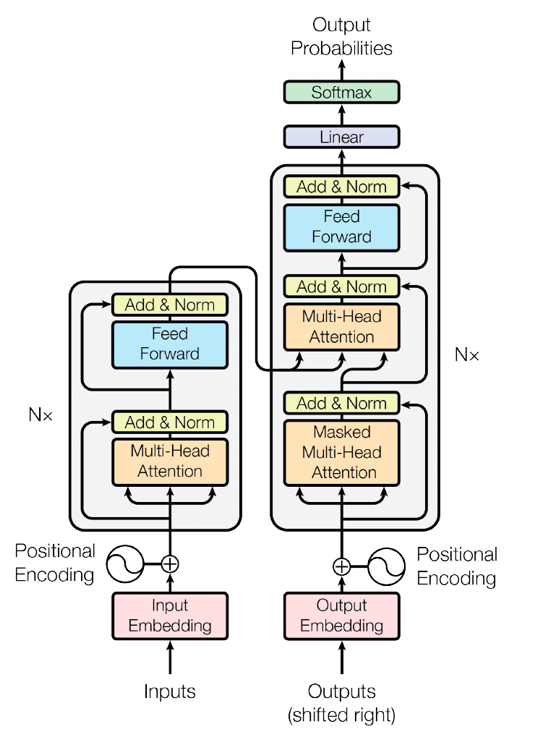
\includegraphics[width=0.45\textwidth]{transformer.png}
    \hfill
    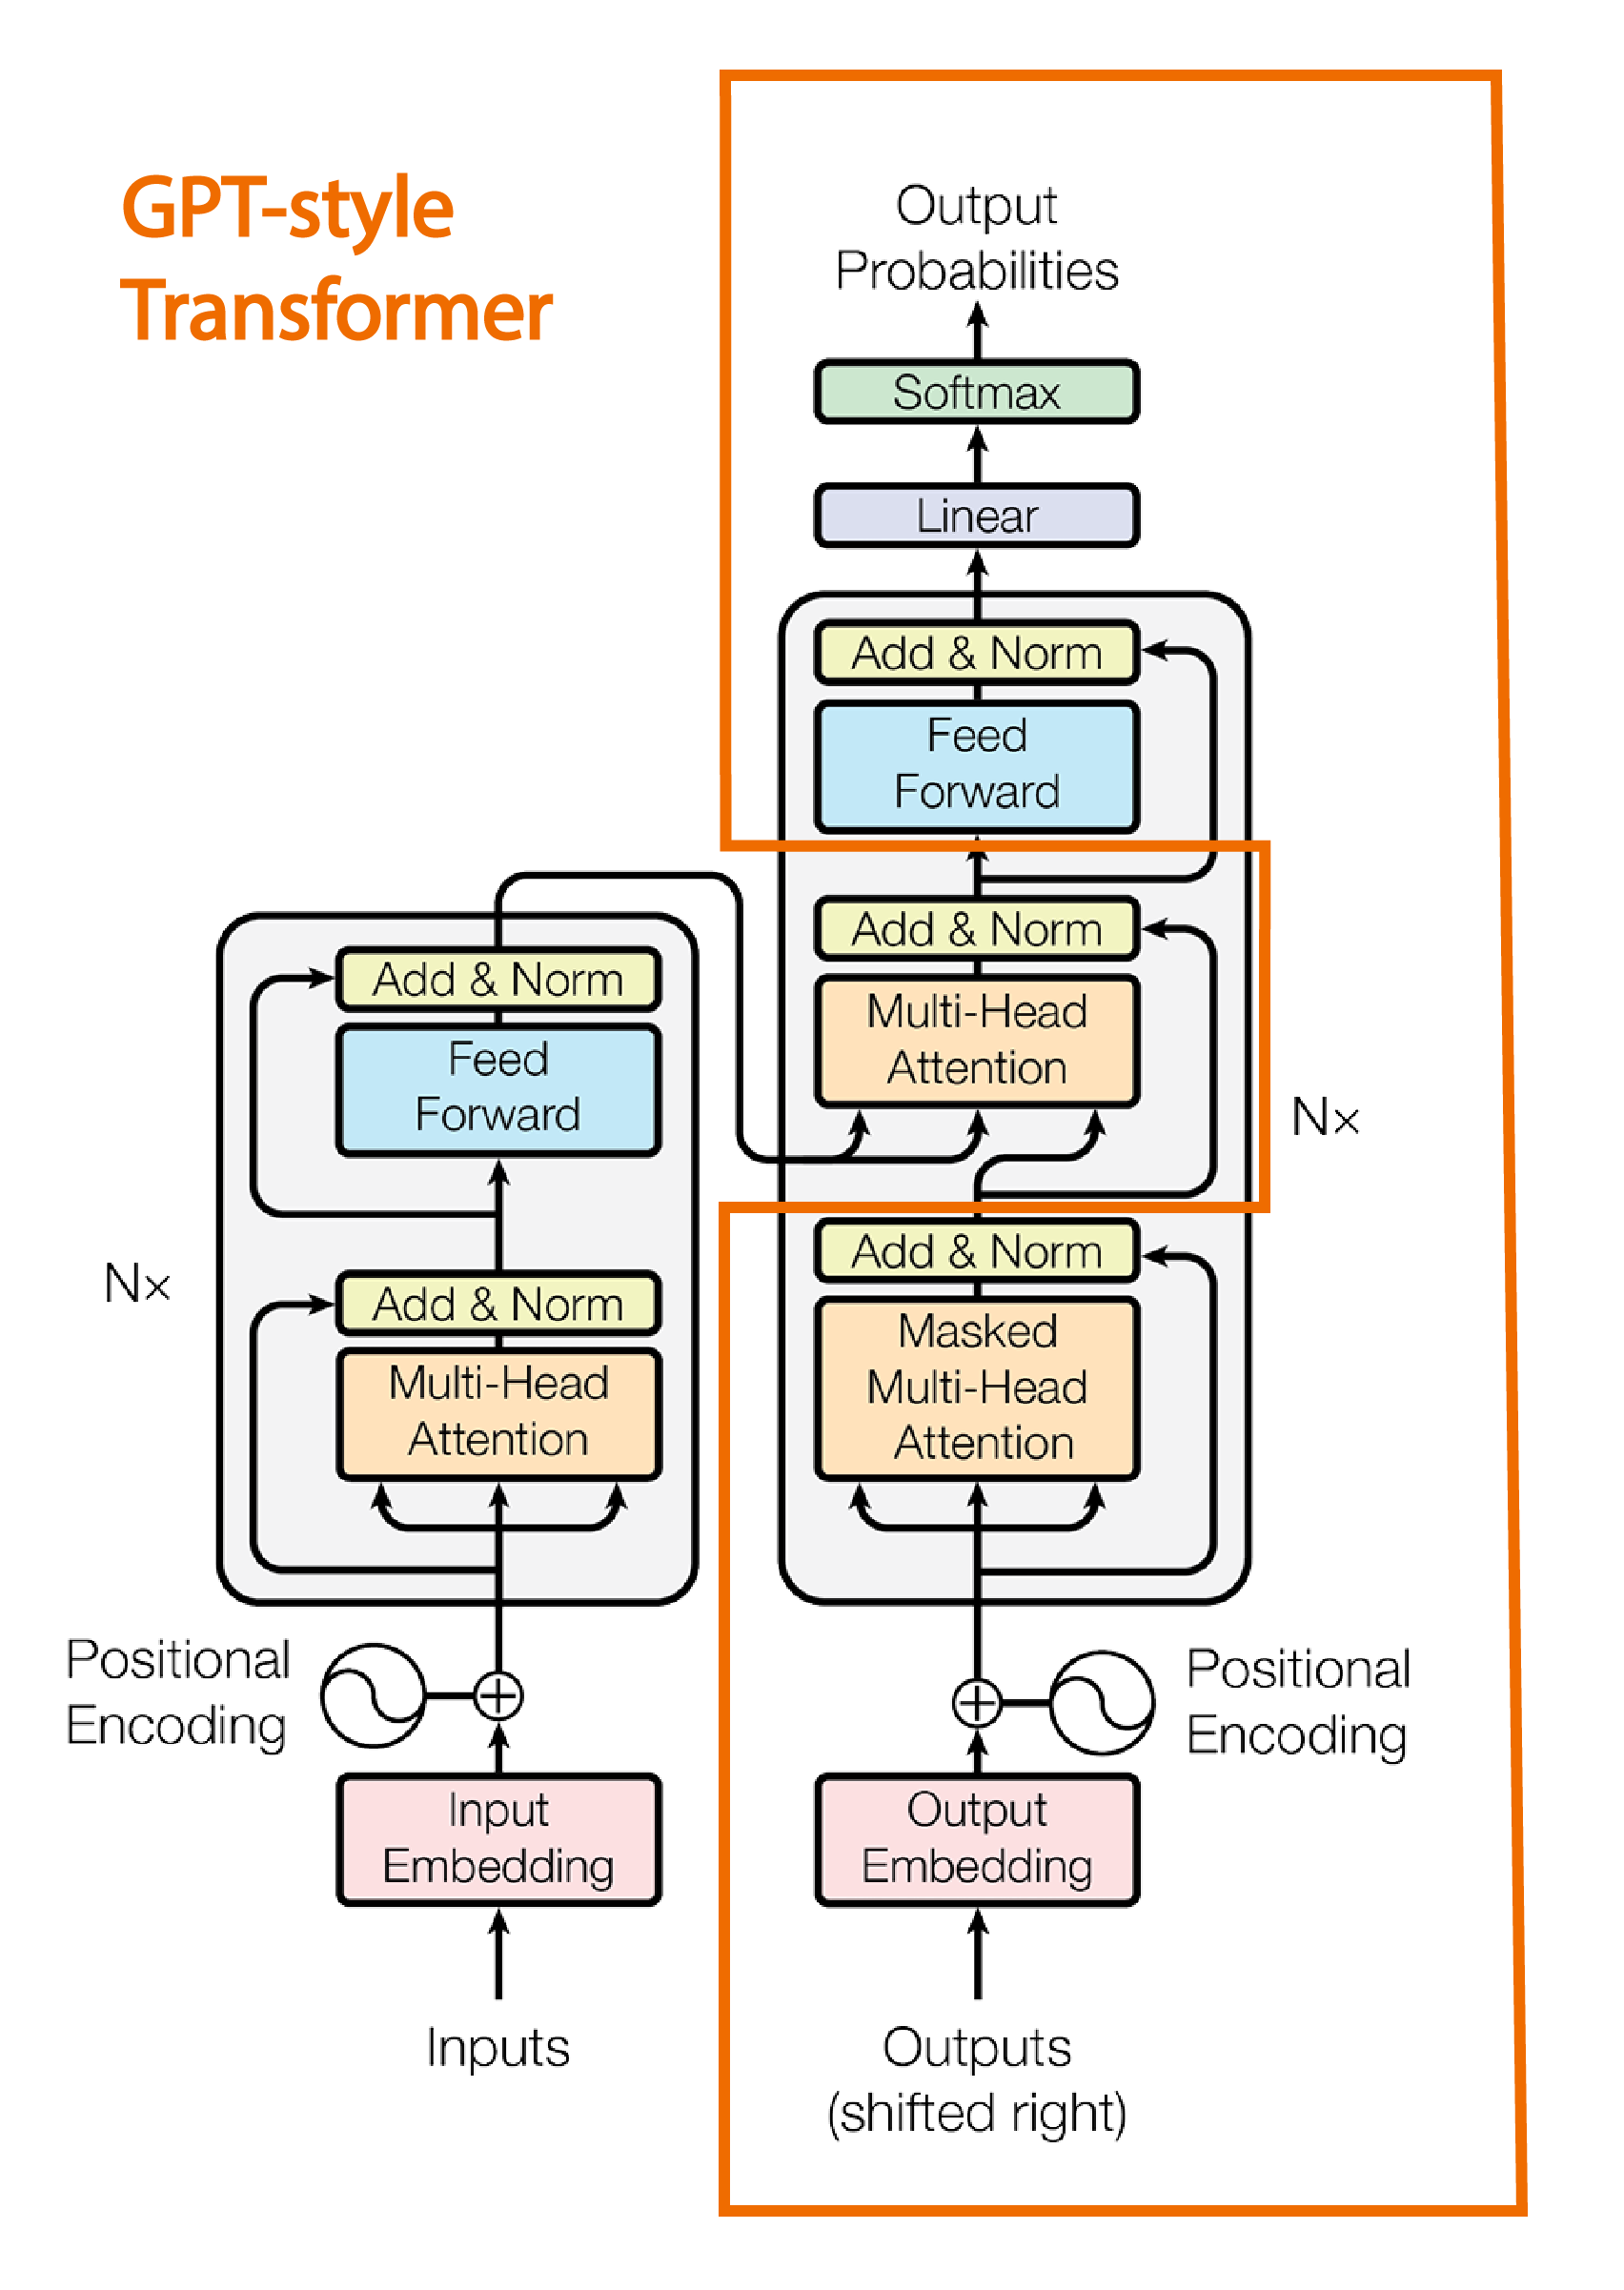
\includegraphics[width=0.45\textwidth]{transformer-gpt.png}
    \caption{On the left, a standard Transformer architecture, which consists of an encoder and a decoder. On the right, we can observe the same architecture, while highlighting the only the layers used by a GPT-style model, which is a decoder-only transformer. The main difference is that the decoder does not attend to the encoder's output, allowing for auto-regressive generation.}
    \label{fig:sidebyside}
\end{figure}

\section{A look at the target hardware} \label{target_hardware}

\section{Relevant compression and optimization techniques}
speak about distillation, paper about width+depth pruning.


